\documentclass[../../main]{subfiles}
\begin{document}

\subsection{Backend architecture}
\label{ss:backend-architecture}

Like we wrote in \ref{ss:overall-system-architecture}, we designed also the backend of our system to support the functionalities the application offers.
A quick overview of the backend can be seen in the following diagram:
\begin{figure}[h]
    \centering
    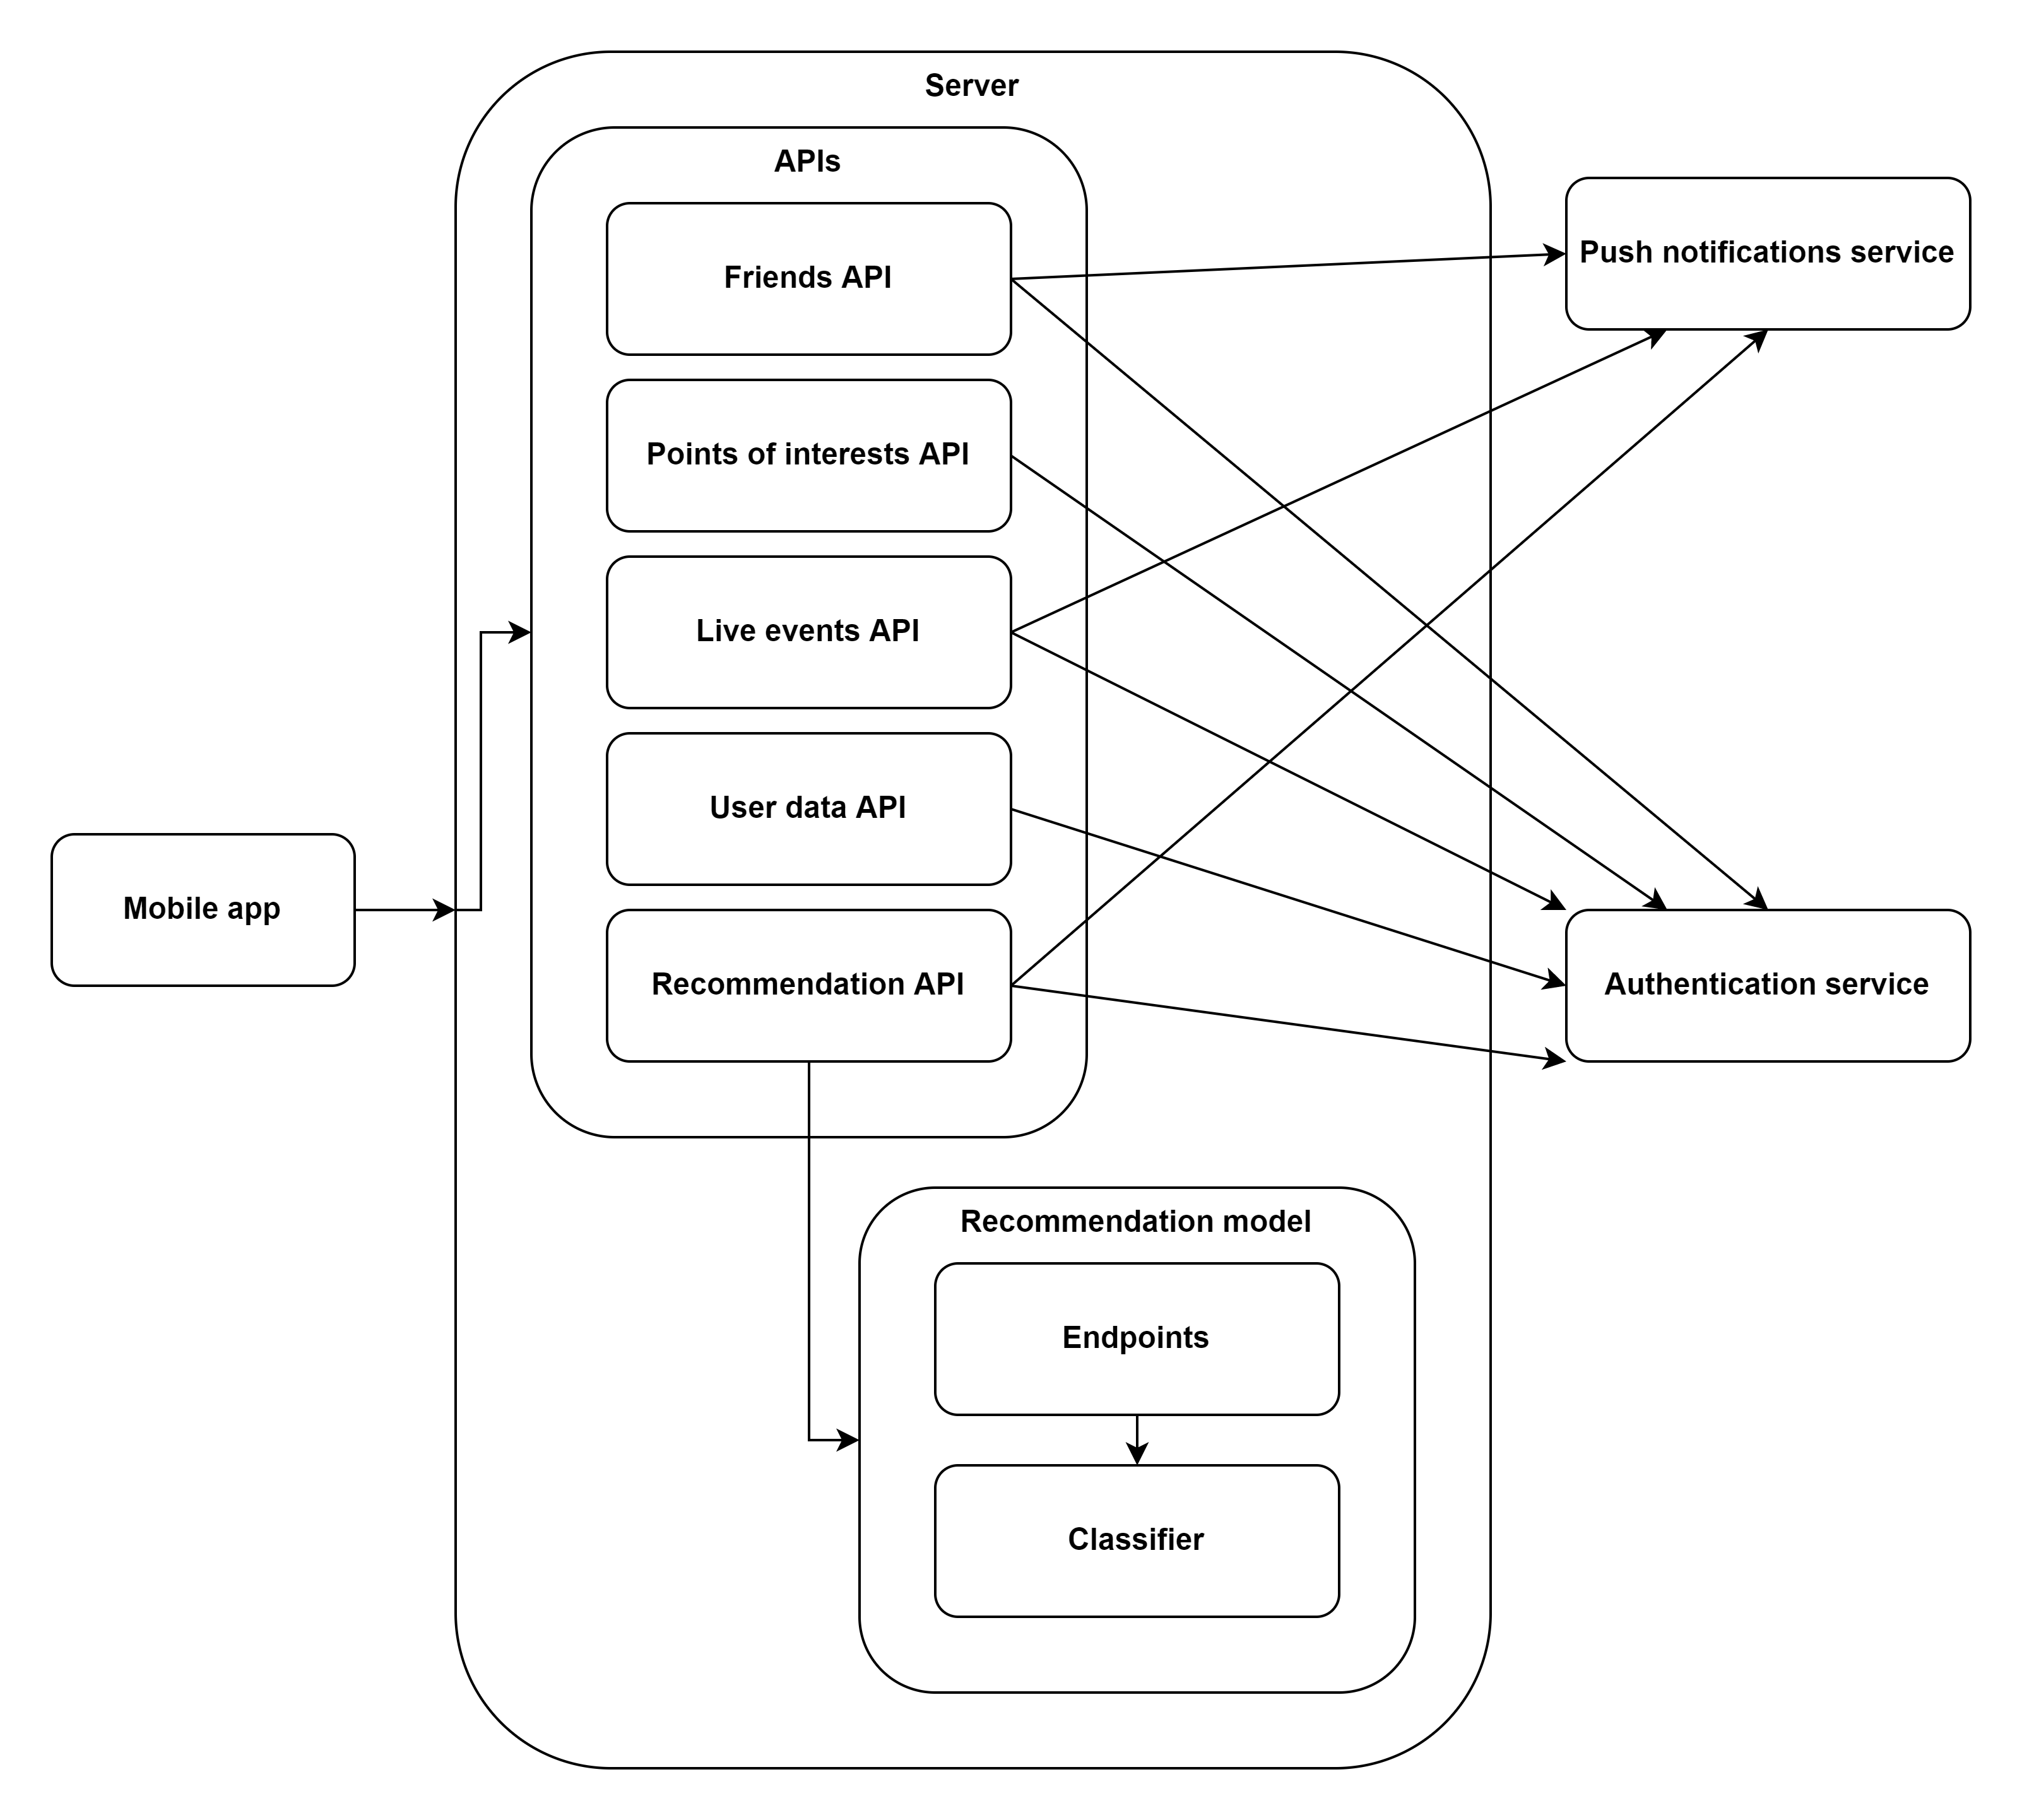
\includegraphics[width=0.8\textwidth]{images/backend_architecture}
    \caption{Backend Architecture}\label{img:backend_architecture}
\end{figure}
The backend architecture is composed by two main parts:
\begin{itemize}
    \item \textbf{APIs}, designed to satisfy all the requests coming from the mobile app;
    \item \textbf{Recommendation model}, which is a service that runs the classifier that generates recommendations given inputs by the APIs.
\end{itemize}

\label{sss:apis}
\subsubsection{APIs}
The Application Programming Interfaces of the backend handle all the incoming requests from the application.\\
We can subdivide them into five main subjects:
\begin{itemize}
    \item \textbf{Friends API}, they enable users to send, accept, or deny friend requests and to retrieve their list of friends;
    \item \textbf{Points of interest API}, they enable users to add or remove pois from their poi list, retrieve their poi list and that of other friends;
    \item \textbf{Live Events API}, they enable users to add live events to the their live events list, retrieve their live event list;
    \item \textbf{User data API}, they enable users to send the backend their authentication and push notification tokens;
    \item \textbf{Recommendation API}, they enable users to register for receiving recommendation for generic places (i.e., pois) or for places of a specific category and to send data that enable the classifier to train again and improve its accuracy.
\end{itemize}
The external \textbf{Authentication service} is called for every API request coming from the users in order to verify if they have rights to perform certain operations or, in general, if they have rights to contact the server at all.
Finally, the \textbf{Push notifications service} is called in the scenarios we already mentioned:
\begin{itemize}
    \item when a new friendship request is sent to a user or confirmed;
    \item when a friend publishes a new live event;
    \item when a periodic recommendation request or recommendation for a place of a specific category were received and thus need to be managed;
    \item when the recommendation model retrained\footnote{It is a useful feature while developing, but it could actually be removed with a more mature release of the application and the system in its whole.}
\end{itemize}

\label{sss:recommendation-model}
\subsubsection{Recommendation model}
The recommendation model part of the backend handles all the requests coming from the \textbf{Recommendation API}.\\
It acts as an interface to the classifier, which will be explained more in detail in \ref{ss:recommendation-model}.


\end{document}